\documentclass[11pt]{article}
%\setlength{\textheight}{20cm} \setlength{\textwidth}{17cm}
%\setlength{\hoffset}{-2cm} \setlength{\voffset}{-2cm}
\usepackage[margin=2.4cm]{geometry}

\usepackage{graphicx}
\graphicspath{{./images}}
\usepackage{amsmath,amsthm,latexsym,amsfonts,amssymb,mathrsfs}
\usepackage[usenames]{color}
\usepackage{tikz}
\usetikzlibrary{math}

\usepackage{cancel,soul,ulem}

\usepackage{url}
%\usepackage[usenames]{color}
\newcommand{\todo}[1]{{\color{red}{#1}}}
\newcommand{\thanh}[1]{{\color{green}{#1}}}
\newcommand{\josef}[1]{{\color{blue}{#1}}}
\newcommand{\thong}[1]{{\color{purple}{#1}}}

\def\IN{\mathbb{N}}
\def\N{\mathbb{N}}
\newcommand{\calO}{\mathcal{O}}
\newcommand{\calB}{\mathcal{B}}
\newcommand{\calBhat}{\hat{\mathcal{B}}}
\newcommand{\calL}{\mathcal{L}}
\newcommand{\I}{\mathcal{I}}
\newcommand{\bfL}{\mathbf{L}}
\newcommand{\bfH}{\mathbf{H}}

\newcommand{\lb}{[\hspace{-0.02in}[}
\newcommand{\rb}{]\hspace{-0.02in}]}
\newcommand{\vk}{{\bf K}}
\newcommand{\ve}{{\bf e}}
\newcommand{\vf}{{\bf f}}
\newcommand{\vn}{{\bf n}}
\newcommand{\vu}{{\bf u}}
\newcommand{\vv}{{\bf v}}
\newcommand{\vs}{{\bf s}}
\newcommand{\calE}{{\mathcal  E}}
\newcommand{\calF}{{\mathcal  F}}
\newcommand{\bchi}{\boldsymbol \chi}
\newcommand{\bphi}{\boldsymbol \phi}
\newcommand{\bpsi}{\boldsymbol \psi}
\newcommand{\bvphi}{\boldsymbol \varphi}
\newcommand{\balpha}{\boldsymbol \alpha}
\newcommand{\bbeta}{\boldsymbol \beta}
\newcommand{\vV}{{\bf V}}
\newcommand{\vH}{{\bf H}}
\newcommand{\vVhat}{\mathbf{\hat V}}
\newcommand{\vHhat}{\mathbf{\hat H}}
\newcommand{\vw}{{\bf w}}
\newcommand{\bH}{{\boldsymbol{H}}}
\newcommand{\bsd}{{\boldsymbol{d}}}
\newcommand{\bsx}{{\boldsymbol{x}}}
\newcommand{\bsy}{{\boldsymbol{y}}}
\newcommand{\bsz}{{\boldsymbol{z}}}
\newcommand{\bsr}{{\boldsymbol{r}}}
\newcommand{\veta}{\boldsymbol{\eta}}
\newcommand{\vsigma}{\boldsymbol{\sigma}}
\newcommand{\vxi}{\boldsymbol{\xi}}
\newcommand{\R}{\mathbb{R}}
\newcommand{\ddiv} {\mathrm{div\;}}
\newcommand{\tr} {\mathrm{tr\;}}
\newcommand{\eps}{\varepsilon}
\newcommand{\calS}{\mathcal{S}}
\newcommand{\calC}{\mathcal{C}}
\numberwithin{equation}{section}
\newcommand{\bsnu}{{\boldsymbol{\alpha}}}
\newcommand{\veps}{{\boldsymbol{\varepsilon}}}
\newcommand{\iprod}[1]{\langle#1 \rangle}
\newcommand{\ud}{\mathrm{d}}
\newcommand{\diam}{\mathrm{diam}}
%\theoremstyle{plain}
\newtheorem{theorem}{Theorem}[section]
\newtheorem{prop}[theorem]{Proposition}%[section]
%\newtheorem{problem}[theorem]{Problem}[section]
\newtheorem{lemma}[theorem]{Lemma}
\newtheorem{corollary}[theorem]{Corollary}
\newtheorem{proposition}[theorem]{Proposition}
\newtheorem{assumption}{Assumption}
%\theoremstyle{definition}
\newtheorem{definition}{Definition}[section]
%\theoremstyle{remark}
\newtheorem{remark}{Remark}[section]


\title{A Locking-free modified conforming FEM for planar elasticity\thanks{School of Mathematics and Statistics, University of New South Wales, Sydney, Australia}\thanks{This work was supported by the Australian Research Council
grant DP220101811.}}
\author{K. Mustapha, W. McLean, J. Dick and  Q. T. Le Gia}
\begin{document}
\maketitle
\begin{abstract}
Due to the divergence-instability, the accuracy of low-order
conforming finite element methods (FEMs) for nearly incompressible elasticity
equations deteriorates as the Lam\'e parameter~$\lambda\to\infty$, or
equivalently as the Poisson ratio $\nu\to1/2$.  This effect is known
as \emph{locking} or \emph{non-robustness}. For the piecewise linear case, the
error in the $L^2$-norm of the standard Galerkin conforming FEM is bounded
by~$C\lambda h^2$, resulting in poor accuracy for practical values of~$h$ if
$\lambda$ is sufficiently large. In this short paper, we show that for 2D
problems the locking phenomenon can be controlled by replacing
$\lambda$ with~$\lambda_h=\lambda/(1+\lambda h)$ in the stiffness matrix. We
prove that with this modification, the error in the $L^2$-norm is bounded
by~$Ch$ for a constant $C$ that does not depend on~$\lambda$.  Numerical
experiments confirm this convergence behaviour and show that, for
practical meshes, our  method is more accurate than the standard method if the
material is nearly incompressible.  Our analysis also shows that the error in
the $H^1$-norm is bounded by $Ch^{1/2}$, but our numerical experiments suggest
that this bound is not sharp.
\end{abstract}
\section{Introduction}

Consider the following linear elasticity equation 
\begin{equation}
 -\nabla \cdot \vsigma(\vu(\bsx)) = \vf(\bsx) \quad \text{for $\bsx \in \Omega\subseteq\R^2$,}
\label{eq:L1}
\end{equation}
subject to homogeneous Dirichlet boundary conditions $\vu = {\bf 0}$ on the
polygonal boundary~$\Gamma:=\partial \Omega$. The   Cauchy stress
tensor~$\vsigma \in [L^2(\Omega)]^{2\times 2}$ is defined as 
\[\vsigma(\vu) = \lambda \nabla\cdot \vu\, {\bf I} 
+ 2\mu \veps(\vu)\quad\text{on $\Omega$,} \] 
with $\vu$ being the displacement vector field and the symmetric strain 
tensor~$\veps(\vu) := \frac{1}{2} (\nabla \vu + (\nabla \vu)^T)$. Here, $\vf$ is
the body force per unit volume, and ${\bf I}$ is the identity tensor.   The
gradient ($\nabla$) and the divergence ($\nabla \cdot$) are understood to be
with respect to the physical variable~$\bsx \in \Omega$.  The constant Lam\'e
parameters, $\mu$~and $\lambda$, are strictly positive, and we are interested
in the case when the Poisson ratio~$\nu$ of the elastic material
approaches~$1/2$.  Thus, $\lambda$ is large and we are dealing with a nearly
incompressible material. {\color{red} In this case, it is known that the
convergence rate may deteriorate (as it depends on $\lambda$) when conforming
FEMs are employed to approximate the solution of~\eqref{eq:L1}. This issue is
commonly referred to as locking. It has been shown that locking is absent for
polynomials of degree~$\ge 4$ on a triangular mesh~\cite{ScottVogelius1985}.
However, on quadrilateral meshes, locking cannot be  avoided for any polynomial
of degree~$\ge1$~\cite{BabuskaSuri1992}.  In a related result,
Vogelius~\cite{Vogelius1983} proved that the $p$-version of the conforming FEM
on smooth domains is  unaffected by locking. The survey paper of Ainsworth and
Parker~\cite{AinsworthParker2022} illustrates and analyses some of the
surprising effects that can occur when $\lambda$ is very large.}

The locking phenomenon in conforming FEMs has motivated researchers to explore
and develop various  locking-free numerical methods ($h$-, $p$-, and
$hp$-versions, low-order, and high-order) for solving the nearly incompressible
elasticity equation~\eqref{eq:L1}. These methods include  nonconforming FEMs
\cite{ArnoldAwanouWinther2014,BrennerSung1992,ChenRenMao2010,Falk1991,
LeeLeeSheen2003,MaoChen2008,YangChen2010}, conforming-nonconforming mixed
FEMs~\cite{BoffiBrezziFortin2013,
GopalakrishnanGuzman2011,HuShi2008,ZhangZhaoChenYang2018}, the weak Galerkin
FEM~\cite{ChenXie2016,
HuoWangWangZhang2020,HuoWangWangZhang2023,LiuWang2022,WangWangWangZhang2016},
the discontinuous Petrov--Galerkin
method~\cite{BramwellDemkowiczGopalakrishnanQiu2012}, the discontinuous Galerkin
method (with hybridization)~\cite{CockburnSchotzauWang2006,DiPietroNicaise2013,
HansboLarson2002,SoonCockburnStolarski2009,Wihler2006}, and the virtual element
 method~\cite{EdoardoStefanoCarloLuca2020,HuangLinYu2022,VeigaBrezziMarini2013,
ZhangZhaoYangChen2019,ZhaoWangZhang2022}.  It is worth mentioning that most of
these methods are more complicated, both computationally and in their analysis,
than the conforming FEM. Furthermore, these methods become more complicated or
not applicable for the case of an inhomogeneous material, where the Lam\'e
parameters are functions of~$\bsx$.

{\color{red}  Another approach that might be used to avoid locking in the
conforming linear FEM is the so-called reduced integration technique
\cite{HughesCohenHaroun1978,MalkusHughes1978}, in which a finite element
interpolation operator~$\Pi$ has the property~$\nabla\cdot(\Pi \vv)=0$ in
a weak sense whenever $\nabla\cdot\vv=0$.  The same procedure was used in
for the case of a pure traction problem~\cite{BrennerSung1992}. Again,
extending this approach for the case of an inhomogeneous nearly incompressible
material is not feasible.}

The aim of the present work is to demonstrate that the locking phenomenon in
the popular piecewise linear conforming FEM can be avoided by replacing
the Lam\'e parameter~$\lambda$ with~$\lambda_h=\lambda/(1+\lambda h)$ in the
stiffness matrix.  Although most of our analysis is independent of the
dimension, we need to assume that $\Omega\subseteq\mathbb{R}^2$ so that we can
apply certain $H^2$-regularity results
of Brenner~and Sung~\cite{BrennerSung1992}.

In the next section, we succinctly discuss the weak formulation of Problem~\eqref{eq:L1} and the well-posedness of the modified conforming FEM. In Section \ref{ConvAna}, we demonstrate that the 
scheme is $O(h)$~accurate, uniformly in~$\lambda$. Additionally, we include a remark on the applicability of these results in the case of mixed Dirichlet-traction boundary conditions. Furthermore, we include another remark on how to extend the proposed finite element scheme and the convergence analysis for the case of an inhomogeneous body, where  the Lam\'e parameters $\lambda$ and $\mu$ depend on the space variable $\bsx \in \Omega$.  
To support our theoretical findings, we present some numerical results in Section~\ref{Sec: Numeric} for two different examples,  including Cook's benchmark problem.
%%%%%%%%%%%%%%%%%%%%%%%%%%%%%%%%%%%%%%%%%%%%%%%%%%%%%%%%%%%%%%%%%%%%%%%%%%%%%%%%%%%%%
\section{Modified  conforming FEM}\label{Sec: FEM}
In this section, we briefly discuss the existence and uniqueness of the weak solution of \eqref{eq:L1}, and then define our piecewise linear modified conforming Galerkin FEM. We investigate the error estimates in a separate section.  

In the weak formulation of  equation~\eqref{eq:L1}, we seek $\vu \in \vV$ satisfying
\begin{equation}\label{para weak}
 \calB(\vu, \vv) = \ell(\vv), \quad \text{for all~~$\vv \in \vV$,}
\end{equation}
where the linear functional~$\ell$ and the bilinear form~$\calB$ are defined by
\begin{equation*}\label{eq: bilinear}
\ell(\vv) = \int_\Omega \vf \cdot \vv \,\ud\bsx 
 \quad\text{and}\quad
\calB(\vu,\vv)=\int_\Omega[2\mu\,\veps(\vu):\veps(\vv)+\lambda(\nabla\cdot\vu)
(\nabla\cdot\vv)]\,\ud\bsx.
\end{equation*}
The colon operator is the inner product between tensors.  Let $\|\cdot\|$ denote the norm 
in~${\bf L}^2(\Omega)=[L^2(\Omega)]^2$, and let $\|\cdot\|_{\bf V}$~and $\|\cdot\|_{\bf H}$ denote the 
norms in $\vV=[H^1_0(\Omega)]^2$~and ${\bf H}=[H^2(\Omega)]^2$, respectively. Here, $H^1_0(\Omega)$~and 
$H^2(\Omega)$ are the usual Sobolev spaces of scalar-valued functions on~$\Omega$.  Finally, $\vV^*$ is the 
dual space of~$\vV$ with respect to the inner product in~${\bf L}^2(\Omega)$. 
 
Since $\calB(\vv,\vw) \le C_{\lambda,\mu}\|\nabla \vv\|\,\|\nabla \vw\|
\le C_{\lambda,\mu}\| \vv\|_{\vV}\,\|\vw\|_{\vV}$ for $\vv,\vw \in \vV$, the bilinear 
form~$\calB(\cdot,\cdot)$ is bounded over $\vV \times \vV$. The coercivity of~$\calB(\cdot,\cdot)$ 
on~$\vV$ follows from Korn's inequality,
\begin{equation}\label{eq: coer B}
\|\vv\|_\calB^2:=\calB(\vv,\vv)\ge  2 \mu\|\veps(\vv)\|^2 \ge c \mu \| \vv\|_{\vV}^2, 
\quad \vv \in \vV.
\end{equation}
Owing to these two properties, and since $|\ell(\vv)|\le \|\vf\|_{\vV^*}\|\vv\|_{\vV}$,  an application of 
the Lax--Milgram theorem completes the proof of the next theorem.   

\begin{theorem}\label{thm: unique solution}
For every $f \in \vV^*$, the problem~\eqref{para weak} has a unique solution~$\vu\in\vV$. 
\end{theorem}

The convergence analysis rests on balancing two terms that scale differently
with the size of the domain~$\Omega$.  We therefore introduce a reference
domain with unit diameter,
\[
\widehat\Omega=L^{-1}\Omega=\{\,L^{-1}\bsx:\bsx\in\Omega\,\}
\quad\text{where $L=\diam(\Omega)$.}
\]
To each function~$\vv:\Omega\to\mathbb{R}^2$ we associate a
function~$\hat\vv:\widehat\Omega\to\mathbb{R}^2$ defined by
\[
\hat\vv(\hat\bsx)=\vv(\bsx)
    \quad\text{for $\bsx=L\hat\bsx\in\Omega$ and $\hat\bsx\in\widehat\Omega$.}
\]
Denote the Sobolev seminorm by $|\hat\vv|_{r,\Omega}=\bigl(\sum_{|\alpha|=r}
\|\partial^\alpha\vv\|^2\bigr)^{1/2}$, and observe that
\[
\|\vv\|=L\|\hat\vv\|_{\mathbf{L}^2(\widehat\Omega)}
\quad\text{and}\quad
|\vv|_{r,\Omega}=L^{1-r}|\hat\vv|_{r,\widehat\Omega}
\]
because $\ud\bsx=L^2\ud\hat\bsx$~and
$\partial^\alpha\vv(\bsx)=L^{-|\alpha|}\partial^\alpha\hat\vv(\hat\bsx)$.
Equip $\vV$ and $\vH$ with norms given by
\begin{equation}\label{eq: V H norms}
\|\vv\|_{\vV}^2=L^{-2}\|\vv\|_\Omega^2+|\vv|_{1,\Omega}^2
\quad\text{and}\quad
\|\vv\|_{\vH}^2=\|\vv\|_{\vV}^2+L^2|\vv|_{2,\Omega}^2,
\end{equation}
and the corresponding spaces
$\vVhat=[H^1_0(\widehat\Omega)]^2$ and $\vHhat=[H^2(\widehat\Omega)]^2$ with
norms given by
\[
\|\hat\vv\|_{\vVhat}^2=\|\hat\vv\|_{\widehat\Omega}^2
    +|\hat\vv|_{1,\widehat\Omega}^2
\quad\text{and}\quad
\|\hat\vv\|_{\vHhat}^2=\|\hat\vv\|_{\vVhat}^2
    +|\hat\vv|_{2,\widehat\Omega}^2.
\]
In this way,
\[
\|\vv\|_{\vV}=\|\hat\vv\|_{\vVhat}
\quad\text{and}\quad
\|\vv\|_{\mathbf{H}}=\|\hat\vv\|_{\vHhat}.
\]

Since $\veps(\vv)=L^{-1}\veps(\hat\vv)$ and
$\nabla\cdot\vv=L^{-1}\nabla\cdot\hat\vv$, if $\vu\in\vV$ satisfies
\eqref{para weak}, then $\hat\vu\in\vVhat$ will
satisfy
\[
\calBhat(\hat\vu,\hat\vv)=\hat\ell(\hat\vv)
\quad\text{for all $\hat\vv\in\vVhat$,}
\]
where
\[
\hat\ell(\hat\vv) = \int_{\widehat\Omega}L^2\hat\vf\cdot\hat\vv\,\ud\hat\bsx
\quad\text{and}\quad
\calBhat(\hat\vu,\hat\vv)=\int_{\widehat\Omega}
[2\mu\,\veps(\hat\vu):\veps(\hat\vv)+\lambda(\nabla\cdot\hat\vu)
    (\nabla\cdot\hat\vv)]\,\ud\hat\bsx,
\]
Here, $\hat\ell(\hat\vv)=\ell(\vv)\le\|\vf\|\|\vv\|\le L\|\vv\|_{\vV}$ so
$\|\hat\ell\|_{\vVhat^*}=\|\ell\|_{\vV^*}\le L\|\vf\|$. For the convergence
analysis, we require the following regularity properties, which, apart from the
dependence on~$L$, are a special case of a result of
Brenner and Sung~\cite[Lemma~2.2]{BrennerSung1992}

\begin{theorem}\label{lem: vu bound}
Assume that $\Omega$ is a convex polygon in~$\mathbb{R}^2$ and that
$\vf\in\mathbf{L}^2(\Omega)$. Then, the weak solution~$\vu$ of~\eqref{para weak}
satisfies
\begin{equation}\label{a priori}
\|\vu\|_{\vV}+\lambda\|\nabla\cdot\vu\|\le C\|\ell\|_{\vV^*}
\quad\text{and}\quad
\|\vu\|_{\vH}\le CL\|\vf\|.
\end{equation}
In both estimates, the constant~$C$ depends on~$\Omega$~and $\mu$, but is
independent of $\lambda$~and $L$.
\end{theorem}
\begin{proof}
By Korn's inequality, $\calBhat(\hat\vu,\hat\vu)\ge c\mu\|\hat\vu\|_{\vVhat}^2$
for a constant~$c>0$ depending only on~$\widehat\Omega$.  Thus,
\[
c\mu\|\hat\vu\|_{\vVhat}^2\le\calBhat(\hat\vu,\hat\vu)=\hat\ell(\hat\vu)
    \le\|\hat\ell\|_{\vVhat^*}\|\hat\vu\|_{\vVhat}
    \le\|\ell\|_{\vV^*}\|\hat\vu\|_{\vVhat}
\]
and so $\|\vu\|_{\vV}=\|\hat\vu\|_{\vVhat}\le C\mu^{-1/2}\|\ell\|_{\vV^*}$.
There exists $\hat\vw\in\vVhat$ such that
$\nabla\cdot\hat\vw=\nabla\cdot\hat\vu$ in~$\widetilde\Omega$ and
$\|\hat\vw\|_{\vVhat}
\le C\|\nabla\cdot\hat\vu\|_{\mathbf{L}^2(\widehat\Omega)}$; see Arnold et
al.~\cite[Theorem~3.1]{ArnoldEtAl1988} and Brenner and
Sung~\cite[Lemma~2.1]{BrennerSung1992}.  Thus,
\[
\lambda\|\nabla\cdot\hat\vu\|_{\mathbf{L}^2(\Omega)}^2
=\lambda\int_{\widehat\Omega}
    (\nabla\cdot\hat\vu)(\nabla\cdot\hat\vw)\,\ud\hat\bsx
\le\calBhat(\hat\vu,\hat\vw)=\hat\ell(\hat\vw)
\le\|\hat\ell\|_{\vVhat^*}\|\hat\vw\|_{\vVhat}
\le C\|\ell\|_{\vV^*}\|\nabla\cdot\hat\vu\|_{\mathbf{L}^2(\widehat\Omega)},
\]
implying $\lambda\|\nabla\cdot\hat\vu\|_{\mathbf{L}^2(\Omega)}^2
\le C\|\ell\|_{\vV^*}$, which completes the proof of the first
inequality.  The second follows by elliptic regularity:
$\|\vu\|_{\vH}=\|\hat\vu\|_{\vHhat}
\le C\|L^2\hat\vf\|_{\mathbf{L}^2(\widehat\Omega)}=CL\|f\|$.
\end{proof}

\begin{remark}
Our need for \eqref{a priori}  is the only reason that
Theorem~\ref{Convergence theorem} below is restricted to a polygonal domain
in~$\mathbb{R}^2$.
\end{remark}

For the finite element scheme, we introduce as usual a family of regular 
quasi-uniform triangulations~$\mathcal{T}_h$ of the domain~$\Omega$ and let 
$h=\max_{K\in \mathcal{T}_h}(h_K)$, where $h_{K}$ denotes the diameter of 
the element $K$.  The space of polynomials with degree at most~$1$ is denoted  by~$P_1$, and the conforming finite element space is then defined by 
\[\vV_h=\{\,\vw_h \in {\bf V}:\text{$\vw_h |_K \in [P_1]^2$ for all $K \in \mathcal{T}_h$}\,\}.
\]
In the standard conforming FEM we seek $\vu_h \in  \vV_h$ such that
$\calB(\vu_h, \vv_h) = \ell(\vv_h)$ for all $\vv_h \in  \vV_h$. To
avoid locking when~$\lambda$ is large, more precisely,
when~$\lambda$ larger than about~$h^{-1}$, we modify this scheme as
follows: find $\vu_h \in  \vV_h$ such that
\begin{equation}\label{FEM new}
\calB_h(\vu_h,\vv_h)=\ell(\vv_h),\quad\text{for all $\vv_h\in\vV_h$},
\end{equation}
where the bilinear operator~$\calB_h$ is defined in the same way as~$\calB$
in~\eqref{eq: bilinear}, except with~$\lambda_h$ in place of~$\lambda$,
that is,
\begin{equation*}
\calB_h(\vu,\vv)=\int_\Omega[2\mu\,\veps(\vu):\veps(\vv)
    +\lambda_h(\nabla\cdot\vu)(\nabla\cdot\vv)]\,\ud\bsx,
\end{equation*} 
for $\lambda_h$ given by~\eqref{eq: lambda_h} below. The existence and
uniqueness of the solution~$\vu_h$ of~\eqref{FEM new} is guaranteed because the
operator $\calB_h$ is bounded and positive-definite on~$\vV_h$.
The map~$\bsx\mapsto\hat\bsx$ takes the triangulation of~$\Omega$ to a
triangulation of~$\widehat\Omega$ with mesh size~$\hat h=h/L$, and we have
the corresponding finite element space
$\vVhat_h=\{\,\hat\vv_h:\vv_h\in\vV_h\,\}$, with $\hat\vu_h\in\vVhat_h$
satisfying
\[
\calBhat(\hat\vu_h,\vv_h)=\hat\ell(\hat\vv_h)
\quad\text{for $\hat\vv_h\in\vVhat_h$.}
\]

\section{Convergence analysis}\label{ConvAna}
For the error analysis, we use a projection
operator~$\Pi_{\hat h}:\vVhat\to\vVhat_h$ with
the approximation property
\[
\|\hat\vv-\Pi_{\hat h}\hat\vv\|_{\widehat\Omega}
    +\hat h\|\nabla(\hat\vv-\Pi_{\hat h}\hat\vv)\|_{\widehat\Omega}
    \le C\hat h^2\|\hat\vv\|_{\vHhat}.
\]
For the corresponding projection~$\Pi_h:\vV\to\vV_h$ given
by~$\Pi_{\hat h}\hat v(\hat\bsx)=\Pi_hv(\bsx)$, it is easily verified that
\begin{equation} \label{projection estimate}
\|\vv-\Pi_h\vv\|_\Omega+h\|\nabla(\vv-\Pi_h\vv)\|_\Omega
    \le CL^{-1}h^2\|\vv\|_{\vH},
\end{equation}
with the same constant~$C$.
The regularity results in Theorem~\ref{lem: vu bound} imply that
\begin{equation}\label{projection estimate Bh}
\begin{aligned}
\|\vu-\Pi_h \vu\|_{\calB_h}^2&=2\mu\|\veps(\vu-\Pi_h \vu)\|^2
     +\lambda_h\|\nabla \cdot (\vu-\Pi_h \vu)\|^2\\
    &\le C(1+\lambda_h)(L^{-1}h)^2\|\vu\|_{\vH}^2
     \le C\lambda_h h^2\|\vf\|^2,
\end{aligned}
\end{equation}
where $\|\vv\|_{\calB_h}=\sqrt{\calB_h(\vv,\vv)}$ is the norm associated with
the operator~$\calB_h$.

\begin{lemma}\label{lem: balance terms}
$\|\vu_h-\Pi_h \vu\|_{\calB_h}^2\le C\bigl(\lambda_h h^2
    +(\lambda-\lambda_h)^2\lambda_h^{-1}L^2\lambda^{-2}\bigr)\|\vf\|^2$.
\end{lemma}
\begin{proof}
From the weak formulation in \eqref{para weak} and the numerical scheme   in
\eqref{FEM new}, we have the property
\begin{align}\label{equ:Gal ort}
\calB_h(\vu-\vu_h, \vv_h) &= \calB_h(\vu, \vv_h)
    -\calB_h(\vu_h,\vv_h)+\calB(\vu,\vv_h)-\calB(\vu,\vv_h) \nonumber \\
&=\calB_h(\vu,\vv_h)-\calB(\vu,\vv_h)  \nonumber \\
&=\int_\Omega(\lambda_h-\lambda)\nabla\cdot\vu\,\nabla\cdot\vv_h\,\ud\bsx
\quad\text{for all $\vv_h \in \vV_h$.}
\end{align}
Applying the Cauchy--Schwarz inequality, we obtain
\begin{multline*}
\|\vu_h-\Pi_h \vu\|_{\calB_h}^2=\calB_h(\vu-\Pi_h\vu,\vu_h-\Pi_h\vu)
    +\int_\Omega(\lambda-\lambda_h)\,\nabla\cdot\vu\,\nabla\cdot
    (\vu_h-\Pi_h\vu)\,\ud\bsx\\
    \le\tfrac14\|\vu_h-\Pi_h \vu\|_{\calB_h}^2+\|\vu-\Pi_h\vu\|_{\calB_h}^2
    +(\lambda-\lambda_h)^2\lambda_h^{-1}\|\nabla\cdot\vu\|^2
    +\tfrac{1}{4}\lambda_h\|\nabla\cdot(\vu_h-\Pi_h\vu)\|^2.
\end{multline*}
Using $\lambda_h\|\nabla\cdot(\vu_h-\Pi_h\vu)\|^2
\le\|\vu_h-\Pi_h\vu\|_{\calB_h}^2$ and then cancelling the similar terms gives
\[
\|\vu_h-\Pi_h\vu\|_{\calB_h}^2\le2\|\vu-\Pi_h\vu\|_{\calB_h}^2
    +2(\lambda-\lambda_h)^2\lambda_h^{-1}\|\nabla\cdot\vu\|^2.
\]
To complete the proof, combine \eqref{projection estimate Bh}, the regularity
results in Theorem~\ref{lem: vu bound}, and the inequality $\|\ell\|_{\vV^*}
\le CL\|\vf\|$.
\end{proof}

We now choose $\lambda_h$ so that the two terms in the lemma balance:
$\lambda_hh^2=(\lambda-\lambda_h)^2\lambda_h^{-1}L^2\lambda^{-2}$.
Rearranging, $(h/L)^2=(\lambda_h^{-1}-\lambda^{-1})^2$ and so
\begin{equation}\label{eq: lambda_h}
\lambda_h=\frac{\lambda}{1+\lambda h/L}.
\end{equation}

\begin{theorem}\label{Convergence theorem}
Assume that $\Omega\subseteq\mathbb{R}^2$ is a convex polygon, and that
$\vf\in\mathbf{L}^2(\Omega)$. Let $\vu$~and $\vu_h$ be the solutions of problems
\eqref{eq:L1}~and \eqref{FEM new}, and define
$\lambda_h$ by~\eqref{eq: lambda_h}.
Then, there is a constant~$C$ depending on $\widehat\Omega$~and $\mu$, but
independent of $\lambda$, $L$~and $h$, such that
\begin{equation}\label{h1 error}
\|\vu-\vu_h\|_{\calB_h}\le C(Lh)^{1/2}\|\vf\|.
\end{equation}
Moreover, if $\calL:{\bf L}^2(\Omega) \to \R$ is a bounded  linear functional,
so that $|\calL(\vw)|\le \|\calL\|\,\|\vw\|$, then
\begin{equation}\label{convergence calL}
|\calL(\vu_h)-\calL(\vu)|\le C(h+\lambda^{-1})\|\vf\|\|\calL\|.
\end{equation}
\end{theorem}
\begin{proof} 
Our choice of~$\lambda_h$ means that
$\lambda_h h^2=(\lambda-\lambda_h)^2\lambda_h^{-1}L^2\lambda^{-2}
    =\lambda h^2(1+\lambda h/L)^{-1}\le Lh$, and therefore by
Lemma~\ref{lem: balance terms},
\begin{equation}\label{eq: uh Pih u}
\|\vu_h-\Pi_h \vu\|_{\calB_h}^2 \le CLh\|\vf\|^2.
\end{equation}
Using this inequality together with~\eqref{projection estimate Bh} shows
\eqref{h1 error}.

To show the second estimate~\eqref{convergence calL}, we replace $\ell$
with~$\calL$ in \eqref{para weak}, and then, by
Theorem~\ref{thm: unique solution}, there exists a unique~$\vu_{\calL} \in \vV$ satisfying
\begin{equation}\label{weak form uL}
\calB(\vu_{\calL}, \vv) = \calL(\vv)\quad\text{for all $\vv \in \vV$.}
\end{equation}
Furthermore, using  Theorem \ref{lem: vu bound} (with $\vu_{\calL}$ in place of $\vu$), we deduce that  
\begin{equation}\label{regulairty of u_L}
    \|\vu_{\calL}\|_{\vV}+\lambda\|\nabla\cdot \vu_{\calL}\| \le C\|\calL\|_{\vV^*}\quad{\rm and}\quad 
\|\vu_{\calL}\|_{\bf H}\le CL\|\calL\|.
\end{equation}
The modified conforming finite element approximation to~$\vu_{\calL}$ is the
function~$\mathbf{\Theta}_h\in\vV_h$ satisfying
\begin{equation}\label{weak form uL discrete}
\calB_h(\mathbf{\Theta}_h,\vv_h) = \calL(\vv_h)
\quad\text{for all $\vv_h \in\vV_h$.}
\end{equation}
By repeating the arguments that led to~\eqref{h1 error}, and using
\eqref{regulairty of u_L}, we obtain
\begin{equation}\label{projection estimate ucalL}
\|\vu_{\calL}-\mathbf{\Theta}_h\|_{\calB_h}\le C(Lh)^{1/2}\|\calL\|.
\end{equation}

By \eqref{FEM new} and \eqref{weak form uL discrete}, we have
$\calL(\vu_h)=\calB_h(\mathbf{\Theta}_h,\vu_h)
=\calB_h(\vu_h,\mathbf{\Theta}_h)=\ell(\mathbf{\Theta}_h)
=\calB(\vu,\mathbf{\Theta}_h)$, whereas \eqref{weak form uL}~and
\eqref{para weak} imply that
$\calL(\vu)=\calB(\vu_{\calL},\vu)=\calB(\vu,\vu_{\calL})$, so
\[
\calL(\vu)-\calL(\vu_h)=\calB(\vu,\vu_{\calL}-\mathbf{\Theta}_h).
\]
Notice that
\[
\calB(\vw,\vv)-\calB_h(\vw,\vv)
    =\int_\Omega (\lambda-\lambda_h)(\nabla\cdot\vw)(\nabla\cdot\vv)\,\ud\bsx
    \quad\text{for all $\vw$, $\vv\in\vV$,}
\]
so
\[
\calL(\vu)-\calL(\vu_h)
    =\calB_h(\vu,\vu_{\calL}-{\bf\Theta}_h)
    +\int_{\Omega}(\lambda-\lambda_h)(\nabla\cdot\vu)
        (\nabla \cdot(\vu_{\calL}-\mathbf{\Theta}_h))\,\ud\bsx.
\]
By \eqref{weak form uL}~and \eqref{weak form uL discrete} it follows that
\begin{equation}\label{uL relation}
\begin{aligned}
\calB_h(\vu_{\calL}-{\bf\Theta}_h,\vv_h)&=\calB(\vu_{\calL},\vv_h)
   -\calB(\vu_{\calL},\vv_h)+\calB_h(\vu_{\calL},\vv_h)-\calL(\vv_h)\\
   &=-\int_{\Omega}(\lambda-\lambda_h)
    (\nabla\cdot\vu_{\calL})(\nabla\cdot\vv_h)\,\ud\bsx
    \quad\text{for all $\vv_h \in\vV_h$.}
\end{aligned}
\end{equation}
In particular, choosing $\vv_h=\vu_h$, we see that
\begin{align*}
\calB_h(\vu,\vu_{\calL}-\mathbf{\Theta}_h)
    &=\calB_h(\vu-\vu_h,\vu_{\calL}-\mathbf{\Theta}_h)
    +\calB_h(\vu_{\calL}-\mathbf{\Theta}_h,\vu_h)\\
    &=\calB_h(\vu-\vu_h,\vu_{\calL}-{\bf\Theta}_h)
    -\int_{\Omega} (\lambda-\lambda_h)
    (\nabla\cdot\vu_{\calL})(\nabla\cdot\vu_h)\,\ud\bsx
\end{align*}
and hence
\begin{multline}\label{change in lambda 2}
\calL(\vu)-\calL(\vu_h)
    =\calB_h(\vu-\vu_h,\vu_{\calL}-\mathbf{\Theta}_h)
+\int_{\Omega}(\lambda-\lambda_h)
    (\nabla\cdot\vu)\nabla\cdot(\vu_{\calL}-\mathbf{\Theta}_h)\,\ud\bsx\\
    +\int_{\Omega}(\lambda-\lambda_h)(\nabla\cdot\vu_{\calL})\bigl[
    \nabla\cdot(\vu-\vu_h)-\nabla\cdot\vu\bigr]\,\ud\bsx.
\end{multline}
Theorem~\ref{lem: vu bound}~and \eqref{regulairty of u_L} imply that
$\|\nabla\cdot\vu\|\le C\lambda^{-1}L\|\vf\|$~and
$\|\nabla\cdot\vu_{\calL}\|\le CL\lambda^{-1}\|\calL\|$. Thus, from the achieved
estimates in \eqref{h1 error}~and \eqref{projection estimate ucalL}, and
using $\|\nabla\cdot\vv\|\le C\lambda_h^{-1/2}\|\vv\|_{\calB_h}$,
\begin{align*}
|\calL(\vu)-\calL(\vu_h)|
    &\le\|\vu-\vu_h\|_{\calB_h}\|\vu_{\calL}-\Theta_h\|_{\calB_h}
    +C\lambda \|\nabla \cdot\vu\|\|\nabla\cdot(\vu_{\calL}-\Theta_h)\|\\
    &\qquad{}+C\lambda\|\nabla\cdot\vu_{\calL}\|
    \bigl[\|\nabla\cdot(\vu-\vu_h)\|+\|\nabla \cdot\vu\|\bigr]\\
    &=C\bigl((Lh)^{1/2}\|\vf\|\bigr)\bigl((Lh)^{1/2}\|\calL\|\bigr)
    +C(L\|\vf\|)\bigl(\lambda_h^{-1/2}(Lh)^{1/2}\|\calL\|\bigr)\\
    &\qquad{}+C(L\|\calL\|)\bigl[
    \lambda_h^{-1/2}(Lh)^{1/2}\|\vf\|+\lambda^{-1}L\|\vf\|\bigr]\\
    &\le C\bigr(Lh+L\lambda_h^{-1/2}(Lh)^{1/2}+L^2\lambda^{-1}\bigr)
        \|\calL\|\|\vf\|.
\end{align*}
Using $\lambda_h^{-1/2}h^{1/2}\le\frac12\lambda_h^{-1}+\tfrac12h$ and
$\lambda_h^{-1}=h+\lambda^{-1}$, the estimate~\eqref{convergence calL}
follows at once.
\end{proof}

\begin{corollary}\label{cor: L2 H1 errors}
There is a constant~$C$, independent of $\lambda$, such that
\[
\|\vu-\vu_h\|\le C(h+\lambda^{-1})\|\vf\|
\quad\text{and}\quad\|\vu-\vu_h\|_{\vV}\le Ch^{1/2}\|\vf\|.
\]
\end{corollary}
\begin{proof}
By choosing 
$\calL(\vv)=\int_\Omega(\vu-\vu_h)\cdot \vv\,\ud\bsx$ in~\eqref{convergence calL}, we have
\[
\|\vu-\vu_h\|^2=\calL(\vu-\vu_h)=\calL(\vu)-\calL(\vu_h)\le Ch\|\vf\|\|\vu-\vu_h\|,
\]
implying that $\|\vu-\vu_h\|\le C(h+\lambda^{-1})\|\vf\|$.  By
\eqref{eq: coer B}~and \eqref{h1 error},
\[
\|\vu-\vu_h\|_{\vV}^2\le C\|\varepsilon(\vu-\vu_h)\|^2
\le C\|\vu-\vu_h\|_{\calB_h}^2\le Ch\|\vf\|^2,
\]
implying the second estimate.
\end{proof}

\begin{remark}
If we compute $\vu_h$ using the unmodified bilinear form~$\calB$, or in other
words, if $\vu_h$ is the usual finite element solution, then the arguments above
simplify to yield the bounds
\[
\|\vu_h-\vu\|_{\calB}\le\|\vu-\Pi_h\vu\|_{\calB}
\le C\lambda^{1/2}h\|\vf\|
\]
with
\[
|\calL(\vu_h)-\calL(\vu)|\le C\lambda h^2\|\calL\|\|\vf\|
\quad\text{and}\quad
\|\vu_h-\vu\|\le C\lambda h^2\|\vf\|.
\]
It is easily verified that
\[
h+\lambda^{-1}<\lambda h^2\quad\text{if and only if}\quad
\lambda>\frac{1+\sqrt{5}}{2h},
\]
so the modification based on~\eqref{eq: lambda_h} should be
advantageous once $\lambda$ is larger than about~$h^{-1}$.
\end{remark}
\begin{remark}
To discuss mixed boundary conditions, let $\boldsymbol{n}$ denote the outward 
unit normal vector with respect to~$\Omega$. Recall that $\Omega$ is a convex polygonal domain, and let the 
closed line segment~$\Gamma_i$ denote the $i$th edge of the boundary~$\Gamma=\partial\Omega$, ordered 
counterclockwise.  Thus, $\Gamma=\bigcup_{i=1}^m \Gamma_i$ for some finite~$m$. We assume  that 
$u={\bf 0}$ on~$\Gamma_D=\bigcup_{i=1}^{m_0} \Gamma_i$ and that $\vsigma\boldsymbol{n}={\bf g}$ 
on~$\Gamma_N=\bigcup_{m_0+1}^{m} \Gamma_i$.  In other words, homogeneous Dirichlet boundary conditions
apply on~$\Gamma_D$, whereas traction boundary conditions apply on~$\Gamma_N$. The measure of~$\Gamma_D$
must be positive, and the Neumann data~${\bf g}\in{\bf L}^2(\Gamma_2)$.

For $\ell(\vv)=\int_\Omega(\vf\cdot\vv)\,\ud\bsx+\int_{\Gamma_2}({\bf g}\cdot\vv)\,\ud s$, the 
existence and uniqueness theorem (Theorem~\ref{thm: unique solution}) remains valid with 
$|\ell(\vv)|\le C(\|\vf\|_{\vV^*}+\|{\bf g}\|_{{\bf L}^2(\Gamma_2)})\|\vv\|_{\vV}$ and
$\vV=\{\,\vw\in [H^1(\Omega)]^2:\text{$\vw=0$ on $\Gamma_D$}\,\}$. The conforming finite element scheme \eqref{FEM new} is also well-defined if we put
\[\vV_h=\{\,\vw_h\in\vV:\text{$\vw_h|_K\in[P_1]^2$ for all $K\in\mathcal{T}_h$}\,\}.\]
The convergence results in Theorem \ref{Convergence theorem} hold true provided the regularity results 
in Theorem~\ref{lem: vu bound} remain valid. In these two theorems, we anticipate that 
$\|\vf\|_{\vV^*}$~and $\|\vf\|$ should be replaced with 
$\|\vf\|_{\vV^*}+\|{\bf g}\|_{{\bf L}^2(\Gamma_N)}$~and 
$\|\vf\|+\|{\bf g}\|_{[H^{1/2}(\Gamma_N)]^2}$, respectively.  For more details, see for example Arnold and 
Falk~\cite{ArnoldFalk1987}, Brenner and Sung~\cite[Lemma 2.3]{BrennerSung1992}, and Brenner and Scott~\cite[Page 319]{BrennerScott2008}.
\end{remark}




\begin{remark} 
{\color{red} Many natural materials appear macroscopically homogeneous but are actually heterogeneous at the microscopic level, consisting of various constituents or phases. 
%These materials can exhibit different mechanical properties and orientations when examined on a small scale. Features such as layers, fibers, laminates, grains, and distortions in the crystalline lattice, collectively referred to as defects, are examples of these inhomogeneities.
In this remark, we discuss the case of inhomogenous elastic material that is nearly incompressible. We define the variable Lam\'e coefficients $\mu$  and $\lambda$  in terms of the Young’s modulus $E$ and the Poisson ratio $0<\nu<1/2$ via 
\[\mu(\bsx)=\frac{E(\bsx)}{2(1+\nu(\bsx))}~~{\rm and}~~ \lambda(\bsx)= \frac{E(\bsx)\nu(\bsx)}{(1-2\nu(\bsx))(1+\nu(\bsx))}.
\]
Let $\nu_{\min}$ and $\nu_{\max}$ be such that $\nu_{\min}\le \nu(\bsx)\le \nu_{\max}$ for $\bsx \in \Omega.$ Since the Poisson ratio function  $\nu(\bsx)$ approaches $1/2$ (nearly incompressible material), we expect the constants $\nu_{\min}$ and $\nu_{\max}$ to be both closed to $1/2.$ Let $\Lambda =\frac{1}{1-2\nu_{\max}}$ and so, 
\[\lambda= \Lambda \widehat \lambda,\quad{\rm where}~~ \widehat \lambda (\bsx)=\frac{E(\bsx)\nu}{1+\nu}\frac{1-2\nu_{\max}}{1-2\nu}.\]
Indeed, the constant factor $\Lambda$   is expected to be very large (and approaches  infinity for materials which are increasingly incompressible).
 We assume that $0<E_{\min}\le E\le E_{\max}<\infty$  for some positive
constants $E_{\min}$ and $E_{\max}$. The regularity results in Theorem \ref{thm:
unique solution} remains valid in this case with $\Lambda$ in place of
$\lambda$, where  the constant~$C$ depends on~$\Omega$, $\mu$ and $\widehat
\lambda$, but is independent of~$\Lambda$; see Dick et al.~\cite[Theorem
3.2]{Dicketal2024}.
We define the modified conforming FEM as in  \eqref{FEM new} with  
\begin{equation*}
\calB_h(\vu,\vv)=\int_\Omega[2\mu\,\veps(\vu):\veps(\vv)+\Lambda_h
\widehat \lambda  (\nabla\cdot\vu)(\nabla\cdot\vv)]\,\ud\bsx.
\end{equation*} 
For the convergence results, we replace $\lambda_h$ with $\Lambda_h$ in the
statements of Theorem~\ref{Convergence theorem} and
Corollary~\ref{cor: L2 H1 errors}.}
%In the proof of
%Theorem~\ref {Convergence theorem}, we replace $\lambda$ with $\Lambda$ in:
%(1) the functions $\phi,\psi,$ and $\chi,$ (2) the text before \eqref{eq: uh
%Pih u} and after \eqref{h1 error}, and (3) the material after \eqref{change in
%lambda 2}.
\end{remark}

%%%%%%%%%%%%%%%%%%%%%%%%%%%%%%%%%%%%%%%%%%%%%%%%%%%%%%%%%%%%%%%%%%%%%%%%%%%%%%
\section{Scaling effects}
In the foregoing analysis, different terms will scale differently with the size
of~$\Omega$.  To obtain a scale-invariant formula for~$\lambda_h$, let
$L=\diam(\Omega)$ denote the diameter of~$\Omega$,
and define
\[
\widehat\Omega=L^{-1}\Omega=\{\,L^{-1}\bsx:\bsx\in\Omega\,\}
\]
so that $\diam(\widehat\Omega)=1$.  We write the $\mathbf{L}^2$-norms on
$\Omega$~and $\widehat\Omega$ by $\|\cdot\|_\Omega$ and
$\|\cdot\|_{\widehat\Omega}$, respectively. Define the Sobolev seminorm
$|\vv|_{r,\Omega}=\bigl(\sum_{|\alpha|=r}
\|\partial^\alpha\vv\|_{\Omega}^2\bigr)^{1/2}$,
and equip $\vV$ and $\vH$ with the norms given by
\begin{equation}\label{eq: V H norms}
\|\vv\|_{\vV}^2=L^{-2}\|\vv\|_\Omega^2+|\vv|_{1,\Omega}^2
\quad\text{and}\quad
\|\vv\|_{\vH}^2=\|\vv\|_{\vV}^2+L^2|\vv|_{2,\Omega}^2.
\end{equation}
If $\vv(\bsx)=\hat\vv(\hat\bsx)$ for $\bsx=L\hat\bsx$, then
$\partial_i\vv(\bsx)=L^{-1}\partial_i\hat\vv(\hat\bsx)$ and so
$|\vv|_{r,\Omega}=L^{1-r}|\hat\vv|_{r,\widehat\Omega}$.  Thus, if the spaces
$\vVhat=[H^1_0(\widehat\Omega)]^2$ and $\vHhat=[H^2(\widehat\Omega)]^2$ are
equipped with the norms given by
\[
\|\hat\vv\|_{\vVhat}^2=\|\hat\vv\|_{\widehat\Omega}^2
    +|\hat\vv|_{1,\widehat\Omega}^2
\quad\text{and}\quad
\|\hat\vv\|_{\vHhat}^2=\|\hat\vv\|_{\vVhat}^2
    +|\hat\vv|_{2,\widehat\Omega}^2.
\]
then
\[
\|\vv\|_\Omega=L\|\hat\vv\|_{\widehat\Omega},\qquad
\|\vv\|_{\vV}=\|\hat\vv\|_{\vVhat},\qquad
\|\vv\|_{\mathbf{H}}=\|\hat\vv\|_{\vHhat}.
\]
Since $\veps(\vv)=L^{-1}\veps(\hat\vv)$ and
$\nabla\cdot\vv=L^{-1}\nabla\cdot\hat\vv$,
if $\vu\in\vV$ satisfies \eqref{para weak}, then $\hat\vu\in\vVhat$ will
satisfy
\[
\calBhat(\hat\vu,\hat\vv)=\hat\ell(\hat\vv)
\quad\text{for all $\hat\vv\in\vVhat$,}
\]
where
\[
\hat\ell(\hat\vv) = \int_{\widehat\Omega}L^2\hat\vf\cdot\hat\vv\,\ud\hat\bsx
\quad\text{and}\quad
\calBhat(\hat\vu,\hat\vv)=\int_{\widehat\Omega}
[2\mu\,\veps(\hat\vu):\veps(\hat\vv)+\lambda(\nabla\cdot\hat\vu)
    (\nabla\cdot\hat\vv)]\,\ud\hat\bsx,
\]
because $\calB(\vu,\vv)=\calBhat(\hat\vu,\hat\vv)$ and
$\ell(\vv)=\hat\ell(\hat\vv)$. Applying Theorem~\ref{lem: vu bound}
to~$\hat\vu$, we have
\[
\|\hat\vu\|_{\vVhat}+\lambda\|\nabla\cdot\hat\vu\|_{\widehat\Omega}
    \le C\|\hat\ell\|_{\vVhat^*}
\quad\text{and}\quad
\|\hat\vu\|_{\vHhat}\le C\|L^2\hat\vf\|_{\widehat\Omega}.
\]
It follows from $\ell(\vv)=\hat\ell(\hat\vv)$~and
$\|\vv\|_{\vV}=\|\hat\vv\|_{\vVhat}$ that
$\|\ell\|_{\vV^*}=\|\hat\ell\|_{\vVhat^*}$.  Moreover,
$\|\vv\|_\Omega\le L\|v\|_{\vV}$, so
\[
\|\vu\|_{\vV}+\lambda\|\nabla\cdot\vu\|_\Omega\le C\|\ell\|_{\vV^*}
\le CL\|f\|_\Omega
\quad\text{and}\quad
\|\vu\|_{\vH}\le CL\|\vf\|_\Omega,
\]
with~$C$ independent of~$L$.

The map~$\bsx\mapsto\hat\bsx$ takes the triangulation of~$\Omega$ to a
triangulation of~$\widehat\Omega$ with mesh size~$\hat h=h/L$.  Defining
projection $\Pi_{\hat h}\hat v(\hat\bsx)=\Pi_hv(\bsx)$, it is easily verified
that the approximation property
\[
\|\hat\vv-\Pi_{\hat h}\hat\vv\|_{\widehat\Omega}
    +\hat h\|\nabla(\hat\vv-\Pi_{\hat h}\hat\vv)\|_{\widehat\Omega}
    \le C\hat h^2\|\hat\vv\|_{\vHhat}
\]
implies that
\[
\|\vv-\Pi_h\vv\|_\Omega+h\|\nabla(\vv-\Pi_h\vv)\|_\Omega
    \le CL^{-1}h^2\|\vv\|_{\vH},
\]
with the same constant~$C$.  Thus, arguing as in~\eqref{projection estimate Bh},
\[
\|\vu-\Pi_h\vu\|_{\calB_h}^2
    \le C\lambda_h\|\nabla(\vv-\Pi_h\vv)\|_\Omega^2
    \le C\lambda_h(L^{-1}h)^2\|\vu\|_{\vH}^2
    \le C\lambda_hh^2\|\vf\|_\Omega^2,
\]
with $\|\nabla\cdot\vu\|_\Omega\le CL\lambda^{-1}\|\vf\|_{\Omega}$,
so instead of~\eqref{eq: balance terms} we obtain
\begin{align*}
\|\vu_h-\Pi_h \vu\|_{\calB_h}^2&\le C\bigl(\lambda_hh^2
    +(\lambda-\lambda_h)^2\lambda_h^{-1}L^2\lambda^{-2}\bigr)\|\vf\|^2\\
&=CL^2\bigl(\lambda_h\hat h^2
    +(\lambda-\lambda_h)^2\lambda_h^{-1}\lambda^{-2}\bigr)\|\vf\|_\Omega^2,
\end{align*}
now with~$C$ independent of~$L$.  By putting
\begin{equation}\label{eq: lambda_h L}
\lambda_h=\frac{\lambda}{1+\lambda h/L}
\end{equation}
we find $\lambda_h\hat h^2=(\lambda-\lambda_h)^2\lambda_h^{-1}L^2\lambda^{-2}
=\lambda\hat h^2/(1+\lambda\hat h)\le\hat h$ and hence
\[
\|\vu_h-\Pi_h\vu\|_{\calB_h}^2\le CL^2\hat h\|\vf\|_\Omega^2
    =CLh\|\vf\|_\Omega^2.
\]
Since $\lambda_hh^2=L^2\lambda_h\hat h^2\le L^2\hat h=Lh$, it follows that
\[
\|\vu_h-\vu\|\le C(Lh)^{1/2}\|\vf\|_\Omega.
\]

Alternatively, we can derive the same estimate by applying
Theorem~\ref{Convergence theorem} to~$\hat\vu_h$ and concluding that
\[
\|\vu_h-\vu\|_{\calB_h}=\|\hat\vu_h-\hat\vu\|_{\calBhat_h}
    \le C\hat h^{1/2}\|L^2\hat f\|_{\widehat\Omega}=C(Lh)^{1/2}\|f\|_\Omega.
\]
Likewise, by defining $\widehat\calL(\hat\vv)=\calL(\vv)$ and
applying \eqref{convergence calL} to~$\hat\vu_h$, we have
\[
|\calL(\vu_h)-\calL(\vu)|=|\widehat\calL(\hat\vu_h)-\widehat\calL(\hat\vu)|
    \le C(\hat h+\lambda^{-1})\|\hat\vf\|_{\widehat\Omega}\|\widehat\calL\|.
\]
The inequality $|\widehat\calL(\hat\vv)|\le\|\calL\|\|\vv\|_\Omega
=\|\calL\|L\|\hat\vv\|_{\widehat\Omega}$ implies that
$\|\widehat\calL\|\le L\|\calL\|$, whereas
$\|\hat\vf\|_{\widetilde\Omega}=L^{-1}\|\vf\|_\Omega$, so
\[
|\calL(\vu_h)-\calL(\vu)|\le C\biggl(\frac{h}{L}+\frac{1}{\lambda}\biggr)
    \|\vf\|\|\calL\|.
\]
Similarly, by applying Corollary~\ref{cor: L2 H1 errors} to $\hat\vu_h$,
\[
\|\vu_h-\vu\|_\Omega=L\|\hat\vu_h-\hat\vu\|_{\widehat\Omega}
    \le CL(\hat h+\lambda^{-1})\|L^2\hat f\|_{\widehat\Omega}
\]
and
\[
\|\vu_h-\vu\|_{\vV}=\|\hat\vu_h-\hat\vu\|_{\vVhat}
    \le C\hat h^{1/2}\|L^2\hat f\|_{\widehat\Omega}.
\]
Thus,
\[
\|\vu_h-\vu\|_\Omega\le CL^2\biggl(\frac{h}{L}+\frac{1}{\lambda}\biggr)
    \|\vf\|_\Omega
\quad\text{and}\quad
\|\vu_h-\vu\|_{\vV}\le C(Lh)^{1/2}\|\vf\|_\Omega.
\]

%%%%%%%%%%%%%%%%%%%%%%%%%%%%%%%%%%%%%%%%%%%%%%%%%%%%%%%%%%%%%%%%%%%%%%%%%%%%%%
\section{Numerical experiments}\label{Sec: Numeric}
%%%%%%%%%%%%%%%%%%%%%%%%%%%%%%%%%%%%%%%%%%%%%%%%%%%%%%%%%%%%%%%%%%%%%%%%%%%%%%
In this section, we illustrate the theoretical convergence results. Based on 
Corollary~\ref{cor: L2 H1 errors}, we expect to observe $O(h)$~and $O(h^{1/2})$
convergence rates in the ${\bf L}^2(\Omega)$-norm for ${\bf u}$~and
$\nabla\mathbf{u}$, respectively, uniformly in~$\lambda$, provided that all the
imposed assumptions are  satisfied.   The Julia code used in these experiments
is available online~\cite{McLean2024}.  We used the scaled version
of~$\lambda_h$ defined in~\eqref{eq: lambda_h L} with~$L=\diam(\Omega)$.

\paragraph{Example 1.} We chose  $\Omega=(0,\pi)^2$ and chose the body force so
that the exact solution is
\[
\vu(\boldsymbol{x})=\begin{bmatrix}  u_1(x_1,x_2)\\  u_2(x_1,x_2)\end{bmatrix}
=\begin{bmatrix}
\bigl(\cos(2x_1)-1\bigr)\sin(2x_2)\\ \bigl(1-\cos(2x_2)\bigr)\sin(2x_1)
\end{bmatrix}
+\frac{\sin(x_1)\sin(x_2)}{\lambda}\begin{bmatrix}1\\ 1\end{bmatrix},
\quad\bsx=(x_1,x_2).
\]
Notice $\vu=\mathbf{0}$ on~$\partial\Omega$.  We used a family of unstructured
triangulations obtained by uniform refinement of an initial coarse mesh.
Table~\ref{tab: L2 errors} compares the errors and convergence rates in the
${\bf L^2}(\Omega)$-norm of the standard conforming, piecewise-linear
Galerkin FEM (using the original bilinear form~$\calB$) with our modified
conforming scheme~\eqref{FEM new} (using $\calB_h$ depending on~$\lambda_h$).
The number of unknowns in the linear system for each mesh is denoted by~$N_h$.
As~$\lambda$ increases from~$100$ to~$100{,}000$ the material becomes more
nearly incompressible and, as expected, the standard method exhibits poor
convergence. By contrast, our new method achieves $O(h)$ convergence uniformly
in~$\lambda$.
   
Table~\ref{tab: H1 errors} compares the errors in~$\nabla {\bf u}$  for the two
methods.  Once again, our new method is more accurate. In fact, it seems to
achieve $O(h)$ convergence, implying that the second error bound in
Corollary~\ref{cor: L2 H1 errors} is not sharp.

\begin{table}
%\newcommand{\Error}{\textrm{Error}}
\newcommand{\Error}{$\|\vu-\vu_h\|$}
\newcommand{\Rate}{\textrm{Rate}}
\renewcommand{\arraystretch}{1.2}
\caption{Errors and convergence rates for ${\bf u}$ in Example~1.}
\label{tab: L2 errors}
\centering
\texttt{
\begin{tabular}{rc|cc|ccc}
\\\hline
\multicolumn{2}{c|}{$\lambda=100$}&\multicolumn{2}{c|}{$\calB$}&
\multicolumn{3}{c}{$\calB_h$}\\
\hline
$N_h$&$h$&\Error&\Rate&\Error&\Rate&$\lambda_h$\\
\hline
%  132& 0.478& 2.37e+00&      &   8.20e-01&      &   8.5 \\
   586& 0.239& 1.07e+00& 1.146&   3.34e-01& 1.296&  15.7 \\
  2466& 0.119& 3.50e-01& 1.612&   1.36e-01& 1.291&  27.1 \\
 10114& 0.060& 9.79e-02& 1.838&   5.46e-02& 1.321&  42.7 \\
 40962& 0.030& 2.56e-02& 1.933&   2.14e-02& 1.353&  59.8 \\
164866& 0.015& 6.52e-03& 1.975&   8.64e-03& 1.307&  74.9 \\
\hline\\\hline
\multicolumn{2}{c|}{$\lambda=1{,}000$}&\multicolumn{2}{c|}{$\calB$}&
\multicolumn{3}{c}{$\calB_h$}\\
\hline
$N_h$&$h$&\Error&\Rate&\Error&\Rate&$\lambda_h$\\
\hline
%  132& 0.478& 3.60e+00&      &   8.46e-01&      &   9.2 \\
   586& 0.239& 2.96e+00& 0.283&   3.64e-01& 1.218&  18.3 \\
  2466& 0.119& 1.76e+00& 0.748&   1.64e-01& 1.146&  35.9 \\
 10114& 0.060& 7.02e-01& 1.326&   7.65e-02& 1.102&  69.3 \\
 40962& 0.030& 2.15e-01& 1.706&   3.56e-02& 1.105& 129.6 \\
164866& 0.015& 5.86e-02& 1.877&   1.60e-02& 1.150& 229.4 \\
\hline\\\hline
\multicolumn{2}{c|}{$\lambda=10{,}000$}&
\multicolumn{2}{c|}{$\calB$}&\multicolumn{3}{c}{$\calB_h$}\\
\hline
$N_h$&$h$&\Error&\Rate&\Error&\Rate&$\lambda_h$\\
\hline
%  132& 0.478& 3.82e+00&      &   8.49e-01&      &   9.3 \\
   586& 0.239& 3.73e+00& 0.034&   3.67e-01& 1.209&  18.6 \\
  2466& 0.119& 3.42e+00& 0.127&   1.68e-01& 1.127&  37.1 \\
 10114& 0.060& 2.57e+00& 0.409&   8.04e-02& 1.065&  73.9 \\
 40962& 0.030& 1.33e+00& 0.949&   3.92e-02& 1.034& 146.7 \\
164866& 0.015& 4.77e-01& 1.484&   1.93e-02& 1.027& 289.1 \\
\hline\\\hline
\multicolumn{2}{c|}{$\lambda=100{,}000$}&
\multicolumn{2}{c|}{$\calB$}&\multicolumn{3}{c}{$\calB_h$}\\
\hline
$N_h$&$h$&\Error&\Rate&\Error&\Rate&$\lambda_h$\\
\hline
%  132& 0.478& 3.84e+00&      &   8.49e-01&      &   9.3 \\
   586& 0.239& 3.84e+00& 0.003&   3.68e-01& 1.208&  18.6 \\
  2466& 0.119& 3.80e+00& 0.014&   1.68e-01& 1.125&  37.2 \\
 10114& 0.060& 3.66e+00& 0.054&   8.08e-02& 1.061&  74.4 \\
 40962& 0.030& 3.20e+00& 0.194&   3.97e-02& 1.026& 148.6 \\
164866& 0.015& 2.16e+00& 0.569&   1.97e-02& 1.011& 296.8 \\
\hline
\end{tabular}
}
\end{table}

\begin{table}
%\newcommand{\Error}{\textrm{Error}}
\newcommand{\Error}{$\|\nabla\vu-\nabla\vu_h\|$}
\newcommand{\Rate}{\textrm{Rate}}
\renewcommand{\arraystretch}{1.2}
\caption{Errors and convergence rates for $\nabla \vu$ in Example~1.}
\label{tab: H1 errors}
\centering
\texttt{
\begin{tabular}{rc|cc|ccc}
\\\hline
\multicolumn{2}{c|}{$\lambda=100$}&\multicolumn{2}{c|}{$\calB$}&
\multicolumn{3}{c}{$\calB_h$}\\
\hline
$N_h$&$h$&\Error&\Rate&\Error&\Rate&$\lambda_h$\\
\hline
%  132& 0.478& 5.55e+00&      &   2.56e+00&      &   8.5 \\
   586& 0.239& 2.66e+00& 1.063&   1.26e+00& 1.020&  15.7 \\
  2466& 0.119& 1.02e+00& 1.387&   6.18e-01& 1.028&  27.1 \\
 10114& 0.060& 3.83e-01& 1.407&   3.00e-01& 1.044&  42.7 \\
 40962& 0.030& 1.57e-01& 1.291&   1.44e-01& 1.061&  59.8 \\
164866& 0.015& 7.01e-02& 1.161&   6.90e-02& 1.058&  74.9 \\
\hline\\\hline
\multicolumn{2}{c|}{$\lambda=1{,}000$}&\multicolumn{2}{c|}{$\calB$}&
\multicolumn{3}{c}{$\calB_h$}\\
\hline
$N_h$&$h$&\Error&\Rate&\Error&\Rate&$\lambda_h$\\
\hline
%  132& 0.478& 8.31e+00&      &   2.59e+00&      &   9.2 \\
   586& 0.239& 6.83e+00& 0.281&   1.30e+00& 0.993&  18.3 \\
  2466& 0.119& 4.12e+00& 0.730&   6.61e-01& 0.980&  35.9 \\
 10114& 0.060& 1.73e+00& 1.253&   3.37e-01& 0.972&  69.3 \\
 40962& 0.030& 5.96e-01& 1.536&   1.70e-01& 0.982& 129.6 \\
164866& 0.015& 1.96e-01& 1.605&   8.43e-02& 1.015& 229.4 \\
\hline\\\hline
\multicolumn{2}{c|}{$\lambda=10{,}000$}&
\multicolumn{2}{c|}{$\calB$}&
\multicolumn{3}{c}{$\calB_h$}\\
\hline
$N_h$&$h$&\Error&\Rate&\Error&\Rate&$\lambda_h$\\
\hline
%  132& 0.478& 8.82e+00&      &   2.60e+00&      &   9.3 \\
   586& 0.239& 8.62e+00& 0.034&   1.31e+00& 0.989&  18.6 \\
  2466& 0.119& 7.89e+00& 0.127&   6.67e-01& 0.973&  37.1 \\
 10114& 0.060& 5.95e+00& 0.406&   3.44e-01& 0.956&  73.9 \\
 40962& 0.030& 3.14e+00& 0.921&   1.78e-01& 0.948& 146.7 \\
164866& 0.015& 1.20e+00& 1.389&   9.21e-02& 0.952& 289.1 \\
\hline\\\hline
\multicolumn{2}{c|}{$\lambda=100{,}000$}&
\multicolumn{2}{c|}{$\calB$}&
\multicolumn{3}{c}{$\calB_h$}\\
\hline
$N_h$&$h$&\Error&\Rate&\Error&\Rate&$\lambda_h$\\
\hline
%  132& 0.478& 8.88e+00&      &   2.60e+00&      &   9.3 \\
   586& 0.239& 8.86e+00& 0.003&   1.31e+00& 0.989&  18.6 \\
  2466& 0.119& 8.77e+00& 0.014&   6.67e-01& 0.972&  37.2 \\
 10114& 0.060& 8.45e+00& 0.054&   3.44e-01& 0.954&  74.4 \\
 40962& 0.030& 7.39e+00& 0.194&   1.79e-01& 0.944& 148.6 \\
164866& 0.015& 5.01e+00& 0.561&   9.31e-02& 0.943& 296.8 \\
\hline
\end{tabular}
}
\end{table}



\begin{figure}
\begin{center}
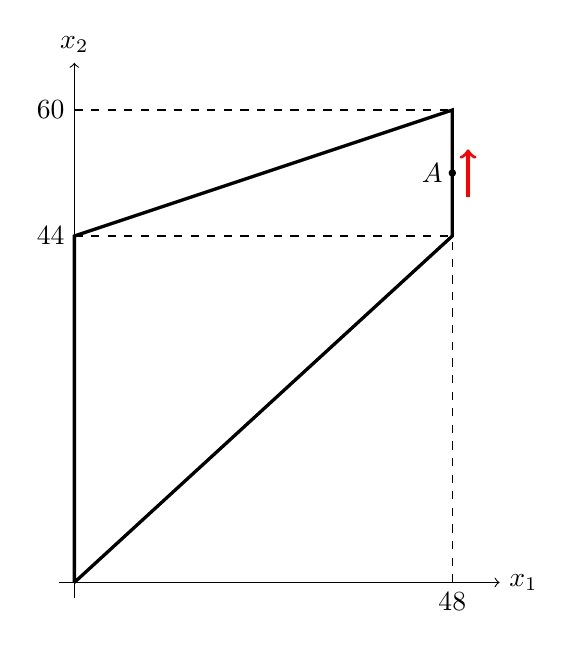
\begin{tikzpicture}[scale=0.1]
\draw[-,very thick] (0,0) -- (48,44) -- (48,60) -- (0,44) -- (0,0);
\node[left] at (0,44) {$44$};
\node[left] at (0,60) {$60$};
\node[below] at (48,0) {$48$};
\draw[->] (-2,0) -- (54,0);
\node[right] at (54,0) {$x_1$};
\draw[->] (0,-2) -- (0,66);
\node[above] at (0,66) {$x_2$};
\draw[dashed] (0,44) -- (48,44);
\draw[dashed] (0,60) -- (48,60);
\draw[dashed] (48,0) -- (48,44);
\node[left] at (48,52) {$A$};
\draw[fill](48,52) circle (0.4);
\draw[->,very thick,red] (50,49) -- (50,55);
\end{tikzpicture}
\end{center}
\caption{The domain $\Omega$ for Cook's membrane problem.}\label{fig: benchmark problem}
\end{figure}

\begin{figure}
\centering
\includegraphics[scale=0.75]{deformed_meshes_978-crop.pdf}
\caption{The deformed mesh obtained when each node is displaced by $\vu_h$.
Left: using the standard conforming method.  Right: using the modified
method~\eqref{FEM new}.}\label{fig: deformed mesh}
\end{figure}

\begin{figure}
\centering
\includegraphics[scale=0.7]{benchmark-crop.pdf}
\caption{Convergence of the computed value of the vertical
displacement~$u_2(A)$ for each choice of the bilinear form.}
\label{fig: benchmark}
\end{figure}
\paragraph{Example 2.} (Cook’s membrane problem \cite{Cook1974}) This is a
benchmark problem for linear elasticity which combines bending and shearing.  As
illustrated in Figure~\ref{fig: benchmark problem}, $\Omega$ is the convex
domain formed by connecting the vertices $(0,0)$, $(48,44)$, $(48,60)$, and
$(0,44)$. The left-hand side of~$\Omega$ is clamped (that is,
$\vu=\mathbf{0}$), and a constant shear load in the vertical direction is
applied on the right-hand side, indicated by the red arrow: $\vsigma \vn =(0,g)$
where $g$ is a positive constant.  The remaining  part of the boundary is
traction-free, that is, $\vsigma \vn=\mathbf{0}$, and the body
force~$\vf=\mathbf{0}$.  The elastic material has Young's
modulus~$E=1.12499998125$ MPa and Poisson ratio~$\nu=0.499999975$, so  the
Lam\'e parameters are
\[
\lambda=\frac{E\nu}{(1+\nu)(1-2\nu)}=7.5\times10^6\quad\text{and}\quad
\mu= \frac{E}{2(1+\nu)}=0.375.
\]
The shear load gives rise to the
functional~$\ell(\vv) = \int_{44}^{60}g v_2\,\ud x_2$, where
$\vv=(v_1,v_2)^T$, $\bsx=(x_1,x_2)$ and $g=1/16$.  Starting from a common
initial mesh with~$h=2.57881$, we solved for~$\vu_h$ using both the
standard bilinear form~$\calB$ (using $\lambda$) and the modified
form~$\calB_h$ (using $\lambda_h=29.796$). Each node was then displaced by the
respective solution~$\vu_h$ to obtain the deformed meshes shown in
Figure~\ref{fig: deformed mesh}.  The locking effect is apparent.

We also compared the computed values for the vertical displacement at the
midpoint~$A=(48,50)$ of the right-hand edge with the benchmark value
$u_2(A)=16.442$~\cite[p.~3491]{LiuWang2022}.  Figure~\ref{fig: benchmark} shows
that using~$\calB$ gives a much less accurate result than using $\calB_h$

%%%%%%%%%%%%%%%%%%%%%%%%%%%%%%%%%%%%%%%%%%%%%%%%%%%%%%%%%%%%%%%%%%%%%%%%%%%%%%%%%%%%%%%%%%%%%
\begin{thebibliography}{99.}
\bibitem{AinsworthParker2022} M. Ainsworth and C. Parker, Unlocking the secrets of locking, Comput. Methods
Appl. Mech. Engrg., 395, 115034 (2022).
\bibitem{ArnoldFalk1987} D. N.  Arnold and R. S.  Falk,  Well-posedness of the fundamental boundary value problems for constrained anisotropic elastic materials, Arch. Rat. Mech. Anal., 98, 143--167 (1987). 

\bibitem{ArnoldEtAl1988} D. N. Arnold, L. Ridgeway Scott and M. Vogelius,
Regular inversion of the divergence operator with Dirichlet boundary conditions
on a polygon, Ann. Scuola Norm. Sup. Pisa Cl. Sci. (4), 15:169--192, 1988.

\bibitem{ArnoldAwanouWinther2014} D. N. Arnold, G. Awanou and  R. Winther, Nonconforming tetrahedral mixed finite elements for elasticity, Math. Models Methods Appl. Sci., 24, 783--796 (2014).

\bibitem{BabuskaSuri1992}  I. Babuška and M. Suri, Locking effects in the finite element approximation of elasticity
problems, Numer. Math., 62, 439--463 (1992).

\bibitem{BoffiBrezziFortin2013} D. Boffi, F. Brezzi and  M. Fortin, Mixed finite element methods and applications. Springer, Berlin (2013).

\bibitem{BrennerScott2008} S. C. Brenner and L. R. Scott, The mathematical Theory of Finite Element Methods, Texts in Applied Mathematics, third edition, Springer, New York, 2008.

\bibitem{BrennerSung1992} S. C. Brenner and  L.-Y. Sung, Linear finite element methods for planar linear elasticity, Math. Comput., 59, 321--338 (1992).

\bibitem{BramwellDemkowiczGopalakrishnanQiu2012} J. Bramwell, L. Demkowicz, J. Gopalakrishnan and  W. Qiu, A locking-free hp DPG method for linear elasticity with symmetric stresses, Numer. Math., 122, 671--707 (2012). 

\bibitem{ChenRenMao2010} S. Chen, G. Ren and  S. Mao, Second-order locking-free nonconforming elements for planar linear elasticity, J. Comput. Appl. Math., 233, 2534--2548 (2010).

\bibitem{ChenXie2016} G. Chen and  X. Xie, A robust weak Galerkin finite element method for linear elasticity with strong symmetric stresses, Comput. Methods Appl. Math., 16, 389--408 (2016).

\bibitem{CockburnSchotzauWang2006} B. Cockburn, D. Schötzau and J. Wang, Discontinuous Galerkin methods for incompressible elastic materials, Comput. Methods Appl. Mech. Eng., 195, 3184--3204 (2006).

\bibitem{Cook1974} R. D. Cook,  Improved two-dimensional finite element, J. Structural. Division., 100, 1851--1863 (1974).

\bibitem{Dicketal2024} J. Dick, Q. T. Le  Gia, W. McLean, K. Mustapha, T. Tran, High-order QMC nonconforming FEMs for nearly incompressible planar stochastic elasticity equations, arXiv preprint arXiv:2402.11545

\bibitem{DiPietroNicaise2013} D. A.  Di Pietro and S. Nicaise, A locking-free discontinuous Galerkin method for linear elasticity in locally nearly incompressible heterogeneous media, Appl. Numer. Math., 63, 105--116 (2013).

\bibitem{EdoardoStefanoCarloLuca2020} A. Edoardo, M. Stefano, L. Carlo and P. Luca,  A dual hybrid virtual element method for plane elasticity problems, ESAIM: Math. Model. Numer. Anal., 54, 1725--1750 (2020).

\bibitem{Falk1991} R. Falk, Nonconforming finite element Methods for the equations of linear elasticity, Math. Comput., 57, 529--550 (1991).

\bibitem{GopalakrishnanGuzman2011} Gopalakrishnan, J., Guzm\'an, J.: Symmetric
nonconforming mixed finite elements for linear elasticity. SIAM J. Numer. Anal.
49, 1504–1520 (2011).

\bibitem{HansboLarson2002} P. Hansbo and  M. G. Larson, Discontinuous Galerkin methods for incompressible and nearly incompressible elasticity by Nitsche’s method, Comput. Methods Appl. Mech. Eng., 191, 1895--1908 (2002).

\bibitem{HuShi2008} J. Hu and Z. C.  Shi,  Lower order rectangular nonconforming mixed finite elements for plane elasticity, SIAM J. Numer. Anal., 46, 88--102 (2008).

\bibitem{HughesCohenHaroun1978}  T. J. R. Hughes, M. Cohen, M. Haroun, Reduced and selective integration techniques in the finite element analysis of plates, Nucl. Eng. Des., 46, 203--222 (1978).

\bibitem{HuoWangWangZhang2020}  F. Huo, R. Wang, Y. Wang and R. Zhang, A locking-free weak Galerkin finite element method for linear elasticity problems,  Computers   Math. Appl., 160, 181--190 (2024).

\bibitem{HuangLinYu2022}  J.G. Huang, S. Lin, Y. Yu, A novel locking-free virtual element method for linear elasticity problems, arXiv:2112.13848v3, 2022.

\bibitem{HuoWangWangZhang2023} F. Huo, R. Wang, Y. Wang and  R. Zhang, An arbitrary order locking-free weak Galerkin method for linear elasticity problems based on a reconstruction operator, (2023).


\bibitem{LeeLeeSheen2003} C.-O. Lee, J. Lee and  D. Sheen, A locking-free nonconforming finite element method for planar linear elasticity, Adv. Comput. Math., 19, 277--291 (2003).

\bibitem{LiuWang2022} Y. Liu and  J. Wang, A locking-free $P_0$ finite element method for linear elasticity equations on polytopal partitions, IMA J. Numer. Anal., 42, 3464--3498, (2022).

\bibitem{MalkusHughes1978} D. S. Malkus, T. J. R. Hughes, Mixed finite element methods — reduced and selective integration techniques: a unification of concepts, Comput. Methods Appl. Mech. Eng., 15, 63--81 (1978).

\bibitem{McLean2024} W. McLean,  \url{https://github.com/billmclean/ControlledLocking.jl.git}, (2024).

\bibitem{MaoChen2008} S. Mao and  S. Chen, A quadrilateral nonconforming finite element for linear elasticity problem, Adv. Comput. Math., 28, 81--100 (2008).

\bibitem{ReddyHuyssteen2019} B. D. Reddy and  D. van Huyssteen, A virtual element method for transversely isotropic elasticity, Comput. Mech., 64, 971--988 (2019).

\bibitem{ScottVogelius1985} L. R. Scott and M. Vogelius, Norm estimates for a maximal right inverse of the divergence operator in spaces of piecewise polynomials, RAIRO Math. Modeling Num. Anal. 19, 111--143 (1985).

\bibitem{SoonCockburnStolarski2009} S.-C. Soon, B. Cockburn and H. K. Stolarski, A hybridizable discontinuous Galerkin method for linear elasticity, Int. J. Numer. Meth.  Eng., 80, 1058--1092 (2009).

%\bibitem{WangQi2004} L.H. Wang, H. Qi, A locking-free scheme of nonconforming rectangular finite element for the planar elasticity, J. Comput. Math., 22, 641--650 (2004).

\bibitem{VeigaBrezziMarini2013} L.B. Da Veiga, F. Brezzi and  L. D. Marini, Virtual elements for linear elasticity problems, SIAM J. Numer. Anal., 51, 794--812 (2013).

\bibitem{Vogelius1983} M. Vogelius, An analysis of the p-version of the finite element method for nearly incompressible materials, Numer. Math., 41, 39--53 (1983).

\bibitem{WangWangWangZhang2016} C. Wang, J. Wang, R. Wang and  R. Zhang, A locking-free weak Galerkin finite element method for elasticity problems in the primal formulation, J. Comput. Appl. Math., 307, 346--366 (2016).

\bibitem{Wihler2006} T. P. Wihler, Locking-free adaptive discontinuous Galerkin FEM for linear elasticity problems, Math. Comp.,  75, 1087--1102 (2006).

\bibitem{YangChen2010} Y. Yang and  S. Chen, A locking-free nonconforming triangular element for planar elasticity with pure traction boundary condition, J. Comput. Appl. Math., 233, 2703--2710 (2010).

%Z. Zhang, Analysis of some quadrilateral nonconforming elements for incompressible elasticity, SIAM J. Numer. Anal. 34 (1997) 640–663

\bibitem{ZhangZhaoChenYang2018} B. Zhang, J. Zhao, S. Chen and  Y. Yang, A locking-free stabilized mixed finite element method for linear elasticity: the high order case, CALCOLO, 55, 1--17 (2018).

\bibitem{ZhangZhaoYangChen2019} B. Zhang, J. Zhao, Y. Yang and  S. Chen, The nonconforming virtual element method for elasticity problems, J. Comput. Phys., 378, 394--410 (2019).

\bibitem{ZhaoWangZhang2022} J. Zhao, T. Wang and  B. Zhang, The stabilized nonconforming virtual element method for linear elasticity problem, J. Sci. Comput., 92, 68, (2022).

\end{thebibliography}

\end{document}
